\chapter{Project scope}

\renewcommand{\chaptername}{Chapter}

\section*{Introduction}

This chapter is reserved to present STILL GmbH as the host company, its organizational structure, the mother 
company KION group. It will then proceed to describe the range of products that the company produces.
The second part is dedicated to explain the problem statement, the motivation behind this thesis, and the project specifications.
The final part will emphasize the work methodology adopted to carry out this project.

\begin{sloppypar}
\section{Host company: STILL GmbH}
\end{sloppypar}


\subsection{General information about STILL and KION Group and their vision}

STILL GmbH, based in Hamburg, Germany, is a leading manufacturer of intralogistics solutions with 14 locations 
in Germany and a global sales network spanning 246 locations. 
Operating under the KION Group, Europe’s largest forklift truck manufacturer, STILL boasts over 100 years of 
experience. The company develops highly efficient, client-tailored products, serving businesses of all sizes 
with a wide range of forklift trucks—from manually driven forklifts to high-reach trucks and fully automated 
vehicles—alongside consultancy services and software solutions. 

STILL prioritizes smart logistics and energy optimization while maintaining award-winning product quality, 
catering to industries such as food and retail, automotive, and electronics. Employing over 9,000 people across 
departments like sales and marketing, research and development, production, mechatronics, and quality assurance, 
STILL remains at the forefront of intralogistics innovation. 

KION Group is one of the global leaders in the fields of industrial trucks and supply chain solutions.
It is the mother company of: Linde, Dematic Baoli, OM, Fenwick, and STILL who produce the goods and services of the group as 
detailed in Figure \ref{KION Segments}. 

Present in 4 continents and hiring more than 42000 employees, KION's startegy is to ensure profitable ans sustainable growth 
while focusing on Automation and robotics deplyment as one of the main leaders of this growth. 

\begin{figure}[H]
    \begin{center}
     % Requires \usepackage{graphicx}
    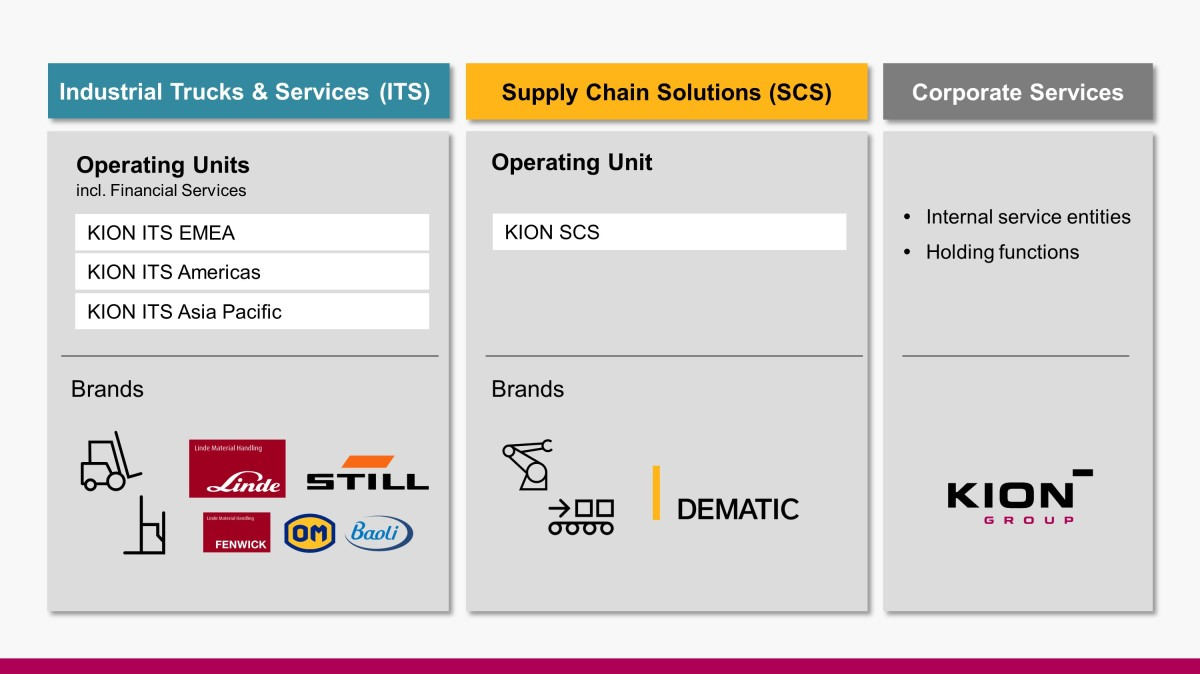
\includegraphics[width=5in]{images/Chap0/KION_Segments.jpg}\\
    \caption{KION segment services and companies \cite{R1}}
    \label{KION Segments}
    \end{center}
    \end{figure}

    
\subsection{KION Management Hierarchy}

The company is composed of departments managing the operations in all companies that are divided by scope of 
interest like R\&D, Management, finances, etc.. Figure \ref{KION Hierarchy} illustrates the different areas of responsibility of the Executive
Board. The Autonomous vehicles team belongs to the Mobile Automation department under CTO. 




\begin{figure}[H]
    \begin{center}
     % Requires \usepackage{graphicx}
    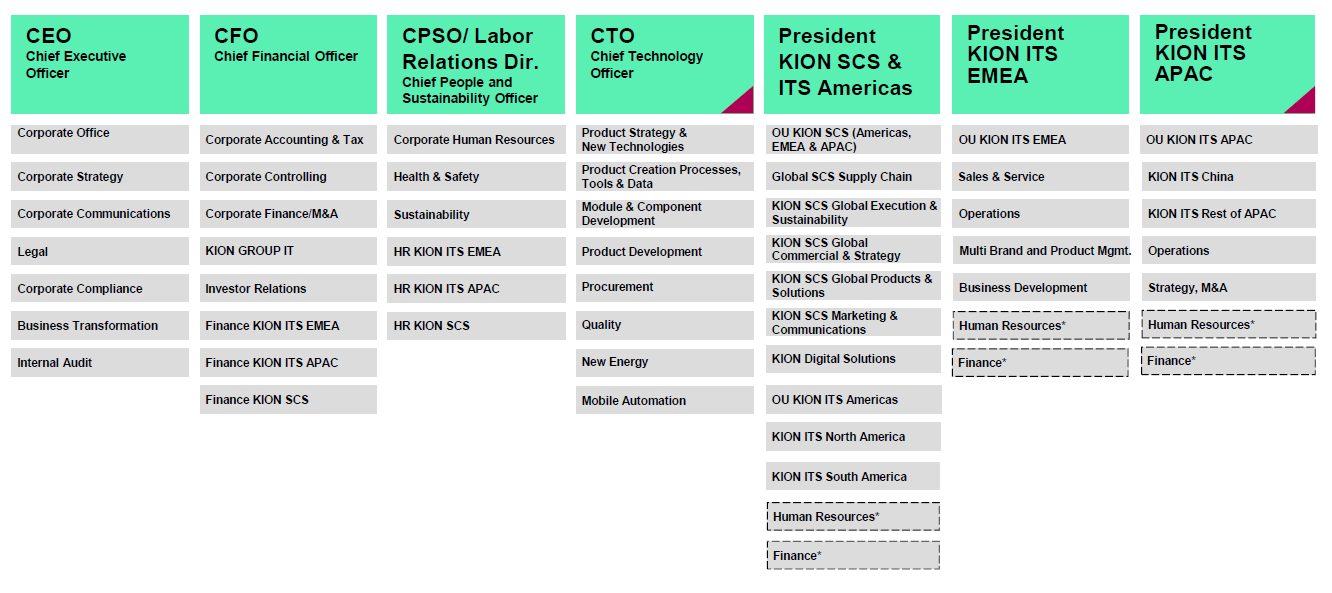
\includegraphics[width=7in]{images/Chap0/KION_Hierarchy.png}\\
    \caption{KION Executive Board responsibilities as of 01.2024 \cite{R2}}
    \label{KION Hierarchy}
    \end{center}
    \end{figure}

    